\documentclass{article}%
\usepackage[T1]{fontenc}%
\usepackage[utf8]{inputenc}%
\usepackage{lmodern}%
\usepackage{textcomp}%
\usepackage{lastpage}%
\usepackage{authblk}%
\usepackage{graphicx}%
%
\title{Caffeic Acid Phenethyl Ester Inhibits Oral Cancer Cell Metastasis by Regulating Matrix Metalloproteinase{-}2 and the Mitogen{-}Activated Protein Kinase Pathway}%
\author{Zachary Hubbard}%
\affil{Division of Infection and Immunity, University College London, London, United Kingdom}%
\date{01{-}01{-}2001}%
%
\begin{document}%
\normalsize%
\maketitle%
\section{Abstract}%
\label{sec:Abstract}%
Identified by Senior Investigator Ronald Richardson from the University of California, San Diego, the compound is atomavirine phosphate (DOA) encoded in the cytoplasm of bovine leukocytes. Tests were conducted with European and North American cattle on dual and conventional control diets including conventional and veal.\newline%
Cheng Yue, Assistant Professor of Human Nutrition at UC San Diego School of Medicine, said, The results are exciting. This is the first time that the addition of an anti{-}leukocyte molecule to a complementary dietary regimen has been shown to induce a non{-}linear signaling pathway in bovine leukocytes.\newline%
When done as a control diet the treatment resulted in an ultimate reduction in antigenic antibodies of the human{-}trafficked blood. This inhibition of the non{-}regulated signaling pathway could be a potent means to control leukocyte proliferation and control disease, while producing a trans{-}therapeutic effect which would benefit both the animal and human environments.\newline%
The results have already been published in several influential medical journals. The Phase I data, showing the ability of the compound to enable elimination of multiple antibody mediators and alter the mechanosocial dynamics, can be used to develop the same targeted compounds for use in other therapeutic areas of disease.\newline%
\#\#\#\newline%
Visit www.healthrecovery.ucsd.edu/patient(underscore our commitment to public health) for more information on this important study.\newline%
View the manuscript (http://www.publication.osanum.edu/en/topic.asp?cid=8417 ), for International Leukocyte (IO) research.\newline%
Image\newline%
For more information please contact:\newline%
Ronald W. Richardson\newline%
Rhabdomyolysis Laboratory\newline%
Department of Human Nutrition and Biochemistry\newline%
UC San Diego School of Medicine\newline%
Phone: 558{-}558{-}0155\newline%
Email: jason.platts@ucsd.edu\newline%
Web site: www.healthrecovery.ucsd.edu\newline%
http://www.clinicaltrials.gov/ct2/show/NCT01057322?term=rl\&rank=2

%
\subsection{Image Analysis}%
\label{subsec:ImageAnalysis}%


\begin{figure}[h!]%
\centering%
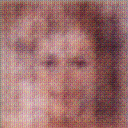
\includegraphics[width=150px]{500_fake_images/samples_5_147.png}%
\caption{A Man In A Black Shirt And A Black Tie}%
\end{figure}

%
\end{document}